\documentclass[12pt]{article}
\usepackage[margin=1in]{geometry}
\usepackage{hyperref}
\usepackage{booktabs}
\usepackage{amsmath, amssymb, amsthm}
\usepackage{enumerate}
\usepackage{graphicx}

\title{Reverse Turing Test: Artificially Generated Text Detector}

\author{Keith Rebello}
%{Northeastern University, Boston, MA}
\date{05/06/2022}

\begin{document}

\maketitle

\abstract
With the development of advanced artificial text generation techniques such as GPT-3, It has become increasingly easier for artificial agents to develop texts that are seemingly indistuingishable from humans. Several efforts have been underway over the last 5 years to look at the development of counteractive tools that differentiate between artificial generated texts and human text. This study aims to look at the ability of classifiers such as logistic regression, decision trees, random forest, and RNNs to differentiate between human generated and artficially generated text. 

\section{Introduction}
Modern natural language generation techniques have surpassed the expectations of the common user. Techniques like GPT-3 have demonstrated the capacity of text agents to develop swathes of text-based content that has not existed before. Such artificially generated texts can be concerning to indviduals as in the wrong hands it can be misused to infiltrate social media platforms, generate large swarms of misinformation, and create harmful texts. Therefore a set of forensic techniques is required to be able differentiate between artificially generated text and human generated text. It is especially important to be able to use such tools to detect shorter tweet-style content which can prevent the spread of bots and chatbots over media platforms. This study aims to develop and compare different classification techniques such as logistic regression, random forest, RNNs and transformers to differentiate between human generated and artficially generated short-length text-content. In this study a comparitive analysis will be done by looking at the capabilities of the aforementioned classifiers at detecting text created by different kinds of text generation techniques such as GPT-2, generic RNNs, LSTMs, and Markov Models.

The primary application of such a classifier would be in detecting generated text on social media platforms such as Twitter or Instagram. Another application would be to detect chatbots. As an alternative application, possibly a future scope, such a detector would also be capable of determining the capability of a conversational agent to carry out a human conversation with a human, without the dependancy on human evaluation or other metrics such as BLEU scores.

\section{Theory}
\subsection{Random Forest Classifier}
Random Forest Classifiers are an ensemble learning based classification technique that builds an ensemble of decision trees and prunes out trees based on a probability-based indexing. In this classification, a sample of the training set is taken at random with replacement and then decision trees are built on it. In addition to this bagging scheme, random forest also performs feature bagging which randomly subsets a set of features to model. After this random forest algorithm acts as a meta-estimator which takes an average score of the decision trees constructed to predict accuracy and prevent over-fitting.

\subsection{Support Vector Machine}
Support Vector Machines are a robust method for classification and are considered to be one of the best models for classification of data. This technique utilizes optimization to classify samples by finding hyperplanes in the feature space  They are particularly robust when handling even non-linearly seperable data by using kernels which transform the non-linear feature space of the sample data to a linear hyperspace. This ability to transform data and to wield convex optimization methods effectively is what leads to a good performance in classification tasks

\subsection{Logistic Regression}
Logistic Regression uses Maximum Likelihood Estimation in order to approximate the probability of an event occuring based on a given dataset. In the case of this study, the logistic regression model aims to model the probability of a binary outcome (bot or human) given the input data as an input variable. The logistic function for the model is of the form:
\begin{equation}
	P(x) = \frac{1}{1+e^{-(x-\mu)/s}}
\end{equation}
Where $\mu$ is a location parameter and s is a scale parameter for x. The combination the location parameter and scale parameter yields a normalized value for x that is then placed in the overaching sigmoid. 

\subsection{Long-Short Term Memory}
Long-Short Term Memory or LSTMs are a popular type of Recurrent Neural Network which are designed with the ability to better deal with sequential data such as text. In order to effectively model sequences, the model needs to be able to handle variable-length sequences, track long-term dependencies, maintain information about the order, and share parameters across the sequence. By using a recurrence mechanism that transfers previous information (or some part of it) from prior nodes in a sequence, they are capable of capturing the influence of time on the sequence. LSTMs are able to achieve this by further introducing specific mechanisms to transfer information across the sequence without falling into issues of vanishing gradients which may occur when dealing with large sequences. They introduce a ‘forget gate’ that decided which information should be forgotten from the previous time-step, an ‘input gate’ that decides how much of the current information should be passed on to the next node,  and an ‘output gate’ that passes combines the previous information with the current information to help decide what information should be used in the next gate.
\begin{equation}
\begin{aligned}
	\textbf{Input Gate: }i_{t} = \sigma(W_i.[h_{t-1},x_t]+b_i) \\
	\textbf{Cell State: }\tilde{C_{t}} = \tanh(W_c.[h_{t-1},x_t]+b_c)\\
	\textbf{Forget Gate: }f_{t} = \sigma(W_f.[h_{t-1},x_t]+b_f)\\
	\textbf{Output Gate: }o_{t} = \sigma(W_o.[h_{t-1},x_t]+b_o)\\
				h_{t} = o_t.\tanh(C_t)
\end{aligned}
\end{equation}


\section{Methodology}
\subsection{Dataset}
The dataset that will be used is the TweepFake dataset from kaggle \cite{noauthor_tweepfake_nodate} which was developed as part of a research study by Fagni et al \cite{fagni_tweepfake_2021}. The dataset consists of 25,838 samples of tweets from Bots and Humans. It is a balanced dataset with 50\% of the tweets coming from human accounts and 50\% coming from Bot accounts.  There are 9 different kinds of techniques of text-generation (GPT-2, RNN, Markov Models, LSTM, Markov Chains,CharRNN, OpenAI, RNN+Markov) employed by this dataset with two unknown text generation methods also included in the dataset. This study looked to simply classify a given text as bot (1) or human (0) and hence the 50-50 split is the most important facet of this dataset. 

\subsection{Model}
For this study, the data handling was carried out using pandas, and numpy libraries. The data exploration additionally used matplotlib. The implementation of support vector machines, logistic regression classifier and random forest classifier was done using the sci-kit learn library in python. The train test split was used to create testing and training data. Gridsearch was used to fine-tune hyperparameters and decide the best combination of various hyperparameters. For the logistic regression, C, which is the inverse of the regularization is hyperparameter which is fine tuned. Similarly in Support Vector Machines, along with the hyperparameter C, kernel choice of 'linear' and 'rbf, and gamma choice of '1e-3' and '1e-4' are fine-tuned. Lastly, for the random forest classifier, the number of estimators, maximum depth of the traversal, minimum sample split and minimum sample leaf size was chosen as the hyperparameters to be fine tuned. The hyperparameters for each classifier is summarized in the table below\ref{table:hyp}. The LSTM was implemented using pytorch.  The dataset and dataloader functions are utilized to effectively feed the training and testing data. The BERT embeddings were implemented using BERTtokenizer and BERTModel from the transformers library. The LSTM model consists of two single layer LSTMs with a dropout of 0.5 to prevent overfitting, which is then connected to linear layer to generate the output which is a confidence score. The model is training for 10 epochs in both the tfidf and BERT cases, with Cross-Entropy Loss being used along with an Adam optimizer with learning rate 1e-4 and weight decay of 1e-5.

\begin{table}[ht]
\begin{tabular}{|l|l|}
\hline
\textbf{Classifier}                & \textbf{Hyper-parameters}                                          \\ \hline
\textbf{Logistic Regression}       & C (regularization)                                                 \\ \hline
\textbf{Support Vector Classifier} & C, kernel, gamma                                                   \\ \hline
\textbf{Random Forest Classifier}  & n\_estimators, max\_depth, min\_samples\_split, min\_samples\_leaf \\ \hline
\end{tabular}
\caption{Hyper-parameters explored for the classifiers.}
\label{table:hyp}
\end{table}

\section{Experimental Results}
This study conducted two conditions for the choice of modeling.  The first was to look at the performance of the data using tokenization and vocabulary building techniques, namely through TFIDF, and look at the performance of the classifiers using the best set of hyperparameters, i.e through gridsearch. The next condition was to utilize transformer based word embeddings which yields tokenization which accounts for the semantic structure of text. The results of this study are therefore presented in two subsections, one which explore the TFIDF results and one which looks at the improvements  (or lack thereof) by using BERT embeddings during pre-processing. 
The code for the project is available at \url{https://github.com/keithRebello/Artificially-Generated-Text-Detector/blob/master/botDetection.ipynb}

\subsection{TFIDF Results}
After using TDIDF to tokenize the data, and running the pre-processed data using the aforementioned setup, the results of the classification is shown in the table below. For the logistic regression the best set of hyperparameters was setting the regularization inverse 'C' to 2. Similarly for the support vector classifier, the best hyperparameters were setting 'C' to 1, 'gamma' to 0.001 and 'kernel' to 'linear' and for random forest classifier the best hyperparameter setup is 'max depth' to 30, 'min samples leaf' to 5, 'min samples split' to 15, and 'n estimators' to 300. Overall, all fours classifiers seem to have a similar score with SVM narrowly beating out the other two by 0.01 in terms of global accuracy. The performance of the models is shown below, \ref{table:tdidf}

\begin{table}[ht]
\begin{tabular}{|l|lll|lll|l|}
\hline
\textbf{Classifier}          & \multicolumn{3}{l|}{\textbf{Bot}}                                                          & \multicolumn{3}{l|}{\textbf{Human}}                                                            & \textbf{Global}   \\ \hline
\textbf{}                    & \multicolumn{1}{l|}{\textbf{Precision}} & \multicolumn{1}{l|}{\textbf{Recall}} & \textbf{F1} & \multicolumn{1}{l|}{\textbf{Precision}} & \multicolumn{1}{l|}{\textbf{Recall}} & \textbf{F1} & \textbf{Accuracy} \\ \hline
\textbf{Logistic Regression} & \multicolumn{1}{l|}{0.72}               & \multicolumn{1}{l|}{0.80}            & 0.76        & \multicolumn{1}{l|}{0.78}               & \multicolumn{1}{l|}{0.68}            & 0.73        & 0.74              \\ \hline
\textbf{Support Vector}      & \multicolumn{1}{l|}{0.71}               & \multicolumn{1}{l|}{0.83}            & 0.77        & \multicolumn{1}{l|}{0.80}               & \multicolumn{1}{l|}{0.66}            & 0.72        & 0.75              \\ \hline
\textbf{Random Forest}       & \multicolumn{1}{l|}{0.69}               & \multicolumn{1}{l|}{0.82}            & 0.75        & \multicolumn{1}{l|}{0.78}               & \multicolumn{1}{l|}{0.64}            & 0.70        & 0.73              \\ \hline
\textbf{LSTM}                & \multicolumn{1}{l|}{0.60}                   & \multicolumn{1}{l|}{0.51}                & 0.55            & \multicolumn{1}{l|}{0.44}                   & \multicolumn{1}{l|}{0.52}                &0.47             & 0.73             \\ \hline
\end{tabular}
\caption{TDIDF results for the classifiers}
\label{table:tdidf}
\end{table}
 For the LSTM the training loss vs the validation loss is shown below.
\\ 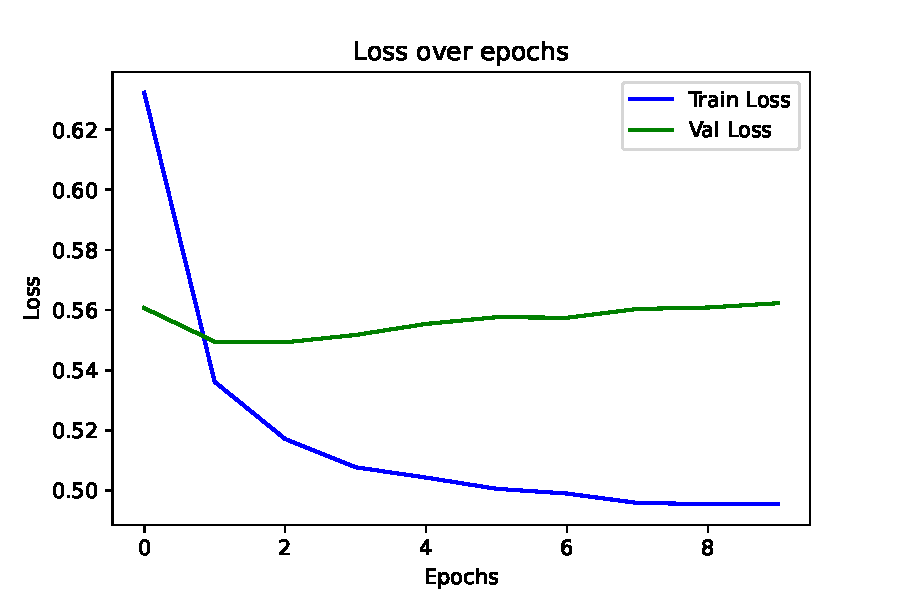
\includegraphics[width=16cm, height=12cm]{tfidf_loss}\\ 

\subsection{BERT Embeddings Results}
Similar to the TFIDF results, the best hyperparameters for logistic regression are 'C'  to 1, for support vector classifier are 'C' to 1, and 'kernel' to 'linear', and for random forest classifier are 'max depth' to 30, 'min samples leaf' to 5, 'min samples split' to 15, and 'n estimators' to 300. The overall performance shows that BERT improves performance by 10 \% in the best case and stays the same in the worst case with LSTM.  The best model overall seems to be SVM in both cases. In this BERT case the performance is 84\% for accuracy. The performance of the models is shown below, \ref{table:bert}
\begin{table}[ht]
\begin{tabular}{|l|lll|lll|l|}
\hline
\textbf{Classifier}          & \multicolumn{3}{l|}{\textbf{Bot	}}                                                          & \multicolumn{3}{l|}{\textbf{Human}}                                                            & \textbf{Global}   \\ \hline
\textbf{}                    & \multicolumn{1}{l|}{\textbf{Precision}} & \multicolumn{1}{l|}{\textbf{Recall}} & \textbf{F1} & \multicolumn{1}{l|}{\textbf{Precision}} & \multicolumn{1}{l|}{\textbf{Recall}} & \textbf{F1} & \textbf{Accuracy} \\ \hline
\textbf{Logistic Regression} & \multicolumn{1}{l|}{0.83}               & \multicolumn{1}{l|}{0.85}            & 0.84        & \multicolumn{1}{l|}{0.85}               & \multicolumn{1}{l|}{0.82}            & 0.84        & 0.84              \\ \hline
\textbf{Support Vector}      & \multicolumn{1}{l|}{0.83}               & \multicolumn{1}{l|}{0.86}            & 0.85        & \multicolumn{1}{l|}{0.86}               & \multicolumn{1}{l|}{0.82}            & 0.84        & 0.84              \\ \hline
\textbf{Random Forest}       & \multicolumn{1}{l|}{0.80}               & \multicolumn{1}{l|}{0.87}            & 0.83        & \multicolumn{1}{l|}{0.86}               & \multicolumn{1}{l|}{0.78}            & 0.82        & 0.83              \\ \hline
\textbf{LSTM}                & \multicolumn{1}{l|}{0.58}                   & \multicolumn{1}{l|}{0.50}                &0.53             & \multicolumn{1}{l|}{0.41}                   & \multicolumn{1}{l|}{0.49}                &0.45             & 0.73              \\ \hline
\end{tabular}
\caption{BERT embedding results for the classifiers}
\label{table:bert}
\end{table}

 For the LSTM the training loss vs the validation loss is shown below.
\\ 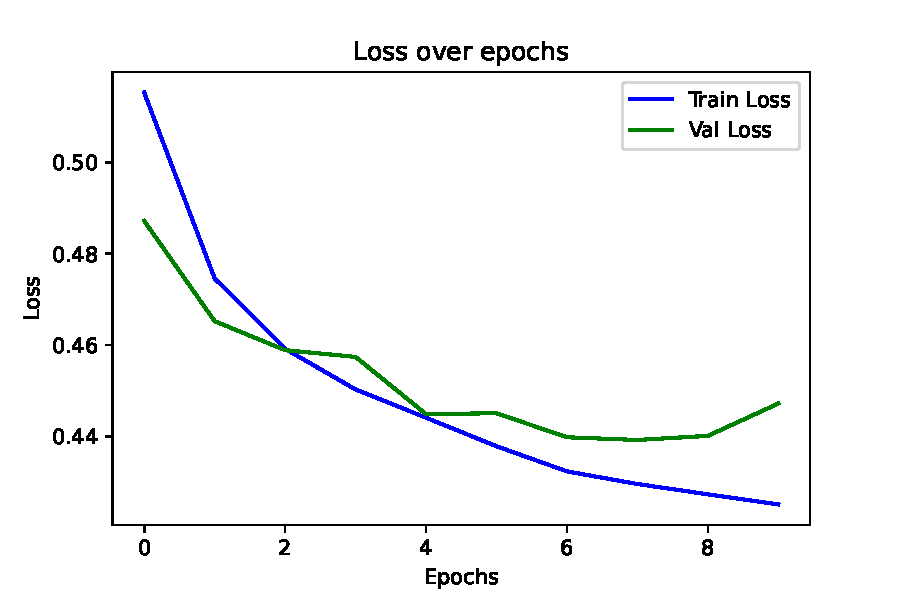
\includegraphics[width=16cm, height=12cm]{bert_loss}\\

\section{Discussion}
From this study we can see that in general popular classifiers are able to do well against a multitude of different writing styles, both human and bot. With a probability better than chance, all these models are able to predict whether a certain text is from a human or a bot. Using BERT embeddings tends to improve the performance of the classifiers in most cases which would indicate that semantic understanding of texts is an important guage when trying to discern whether a certain statement is artificially generated or not. The LSTM model does not seem to improve much when incorporating BERT embeddings, this maybe due to the ability of these systems to already imbue semantic understanding accross the text due to the sequential recurrent nature of the model.

\section{Conclusions}
This study sought to gauge the ability of classifiers to differentiate between text that is generated by human and artificially generated text. By looking at various classifiers such as random forest, support vector machines, logistic regression and LSTMs  this study determined the best performance for the best set up of each classifier through hyper-parameter tuning. Additionally this study also looked the improvement of the models performance when using BERT word embeddings to tokenize the text. It was seen that support vector machines with BERT embeddings is the best model with a global accuracy of 84\%  
\bibliographystyle{plain}
\bibliography{ref}

\end{document}